\documentclass[11pt]{article}
\usepackage[a4paper,margin=1in]{geometry}
\usepackage{amsmath,amssymb,amsthm}
\usepackage{tikz}
\usepackage{booktabs}
\usepackage{xcolor}
\usepackage[hidelinks]{hyperref}
\hypersetup{pdftitle={An integral of hyperbolic tangents},pdfauthor={Vamshi Jandhyala}}
\setlength{\parskip}{0.4em}
\setlength{\parindent}{0pt}

\newtheorem{theorem}{Theorem}
\newtheorem{proposition}[theorem]{Proposition}
\newtheorem{lemma}[theorem]{Lemma}
\newtheorem{corollary}[theorem]{Corollary}

\definecolor{inkblue}{RGB}{40,76,105}
\definecolor{rust}{RGB}{173,80,45}

\title{An integral of hyperbolic tangents: \\ residues, characters and the conductors that occur}
\author{Vamshi Jandhyala}
\date{}

\begin{document}
\maketitle
\vspace{-2em}

\begin{abstract}
For $n\ge2$ let $I_n=\int_0^\infty x^{-2}\tanh(x)\tanh(2x)\cdots\tanh(nx)\,dx$. On Mathematics Stack Exchange it was
observed that for odd $n$ the value is a rational combination of logarithms and values $L'(-1,\psi)$ of even
Dirichlet characters, with coefficients and conductors that look patternless, and asked for a general reduction.
We give one. The poles of $\prod_{k\le n}(1-q^k)/(1+q^k)$ are simple, at the primitive $2m$-th roots of unity with
$\lfloor n/m\rfloor$ odd, and each residue is an explicit constant times a product of $\rho$ cotangents, where
$\rho=n\bmod m$. Expanding the residues in characters gives every coefficient of $L'(-1,\psi)$ as a finite character
sum. Because a product of $\rho$ of these cotangents equals $\pm$ the product of $m-1-\rho$ of them, only
$\rho'=\min(\rho,m-1-\rho)$ matters, and families with $\rho'=0$ bring no new conductor; this accounts for every
conductor that appears or disappears in the observed lists. The finite trigonometric identities behind the residues
are checked in the Lean proof assistant.
\end{abstract}

\section{The question}

Put $q=e^{-2x}$. Since $\tanh(kx)=(1-q^k)/(1+q^k)$,
\[
I_n=\int_0^\infty \frac{P_n(e^{-2x})}{x^2}\,dx,\qquad P_n(q)=\prod_{k=1}^{n}\frac{1-q^k}{1+q^k}=1+\sum_{N\ge1}c_n(N)\,q^N .
\]
The integrand behaves like $n!\,x^{n-2}$ at $0$ and like $x^{-2}$ at infinity, so $I_n$ converges for $n\ge2$. The
question~\cite{MSE} records that $I_n=-2D_n'(-1)$ for the Dirichlet series $D_n(s)=\sum_{N\ge1}c_n(N)N^{-s}$, that for
even $n$ this gives Clausen values, and that for odd $n$ it gives logarithms and $L'(-1,\psi)$ for even characters
$\psi$:
\begin{align*}
I_3&=\ln\tfrac{27}{4},\\
I_5&=4\ln4-3\ln3-5\ln5+16\,\eta'(-1)+4\,L_8'(-1),\\
I_7&=10\ln5+7\ln7-12\ln3-\tfrac{68}{5}\ln2+20\,L_5'(-1)-4\,L_{12}'(-1),
\end{align*}
with $L_q$ the even real character of conductor $q$. From $n=9$ on, complex characters are needed, and the
conductors that occur are, for $n=9,11,13,15$,
\begin{gather*}
\{1,7,8,12,16\},\qquad\{1,5,7,8,9,16,20\},\\
\{1,5,8,9,11,12,16,20,24\},\qquad\{1,5,7,8,9,11,12,13,20,24,28\}.
\end{gather*}
Conductor $12$ appears, disappears and returns; $16$ is missing at $n=15$ although $1+q^8$ still divides the
denominator. The question asks for the general reduction and its coefficients.

Before reading on, try the smallest case: why does $I_3$ contain no $L$-value at all?

\section{Residues}

The denominator $\prod(1+q^k)$ vanishes only at roots of $-1$, so every pole of $P_n$ is a primitive $2m$-th root
of unity $\zeta=e^{i\pi j/m}$ with $j$ odd and coprime to $m$. We use the angles
\[
x_k=\frac{\pi jk}{2m}\qquad(k\in\mathbb{Z}),
\]
and $\varepsilon_m(j)=1$ for odd $m$, $\varepsilon_m(j)=\tan(\pi j/4)=\pm1$ for even $m$ (the character
$\chi_{-4}$ of $j$).

\begin{theorem}\label{thm:res}
$P_n$ has a pole at $\zeta=e^{i\pi j/m}$ exactly when $\lfloor n/m\rfloor$ is odd, and the pole is simple. Write
$n=(2e+1)m+\rho$ with $0\le\rho<m$. Then
\[
a_m(j):=\lim_{q\to\zeta}\Bigl(1-\frac q\zeta\Bigr)P_n(q)
=\frac2m\cdot\frac{4^e\,e!^2}{(2e+1)!}\cdot(-i)^{m-1}\,\varepsilon_m(j)\prod_{k=1}^{\rho}i\cot x_k ,
\]
and $c_n(N)=\sum a_m(j)\,\zeta^{-N}$ for every $N\ge1$, the sum running over all poles.
\end{theorem}

\begin{proof}
Put $q=\zeta u$ and let $u\to1$. The factor $k$ has a pole when $\zeta^k=-1$, that is when $k$ is an odd multiple of
$m$, and a zero when $\zeta^k=1$, when $k$ is a multiple of $2m$. With $t=\lfloor n/m\rfloor$ there are $\lceil t/2\rceil$
factors of the first kind and $\lfloor t/2\rfloor$ of the second, so the order of the pole is $t\bmod2$. For $t=2e+1$,
a factor of the first kind is $(1+u^k)/(1-u^k)\sim 2/(k(1-u))$ and one of the second is
$(1-u^k)/(1+u^k)\sim k(1-u)/2$. Over $k=(2i+1)m$, $i\le e$, and $k=2im$, $1\le i\le e$, these give
$(2/m)\,4^e e!^2/(2e+1)!$ times $1/(1-u)$.

Every other factor has $\zeta^k\ne\pm1$ and tends to $(1-e^{2ix_k})/(1+e^{2ix_k})=-i\tan x_k$. Their product is
computed by pairing angles: $\tan x_{m-k}=\cot x_k$ because $j$ is odd, and $\tan x_{2m-k}=-\tan x_k$. The first
pairing gives $\prod_{k=1}^{m-1}\tan x_k=\varepsilon_m(j)$, the middle factor $\tan(\pi j/4)$ surviving when $m$ is
even. The second shows that each full period $2mt<k<2m(t+1)$, $k\neq(2t+1)m$, contributes
$\prod_{k=1}^{m-1}(-i\tan x_k)(-i\tan x_{2m-k})=\prod_{k=1}^{m-1}\tan^2x_k=\varepsilon_m(j)^2=1$. What remains is $k=2em+r$ with $1\le r<m$, which
gives $(-i)^{m-1}\varepsilon_m(j)$, and $k=2em+m+r$ with $1\le r\le\rho$, where $\tan x_{m+r}=-\cot x_r$ gives
$i\cot x_r$.

Since $P_n$ has the same degree in numerator and denominator and only simple poles, $P_n(q)=A+\sum a_m(j)/(1-q/\zeta)$
for a constant $A$, and expanding each term as a geometric series gives the coefficients.
\end{proof}

Figure~\ref{fig:poles} shows the poles for $n=9$. The constant and the tangent identities, the assembled product over
all $k\le n$, and the inversion rule below are proved in Lean; the limits of single factors are the elementary
$(1-u^k)/(1-u)\to k$.

\begin{figure}[ht]
\centering
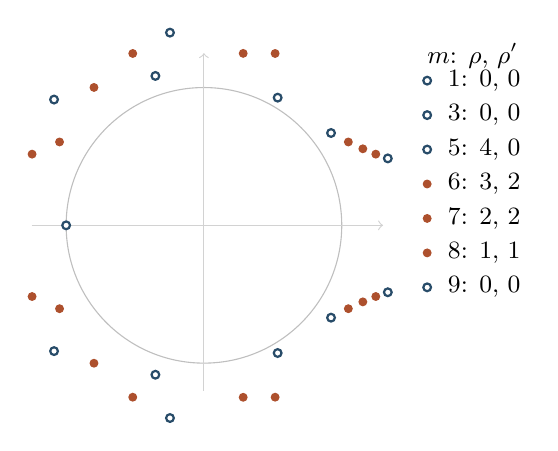
\begin{tikzpicture}[scale=1.75]
  \draw[gray!50] (0,0) circle (1);
  \draw[gray!35,->] (-1.25,0) -- (1.3,0); \draw[gray!35,->] (0,-1.2) -- (0,1.25);
  \draw[fill=white, draw=inkblue, thick] (-1.0000,0.0000) circle (0.028);
  \draw[fill=white, draw=inkblue, thick] (0.5350,0.9266) circle (0.028);
  \draw[fill=white, draw=inkblue, thick] (0.5350,-0.9266) circle (0.028);
  \draw[fill=white, draw=inkblue, thick] (0.9223,0.6701) circle (0.028);
  \draw[fill=white, draw=inkblue, thick] (-0.3523,1.0842) circle (0.028);
  \draw[fill=white, draw=inkblue, thick] (-0.3523,-1.0842) circle (0.028);
  \draw[fill=white, draw=inkblue, thick] (0.9223,-0.6701) circle (0.028);
  \draw[fill=rust, draw=rust] (1.0479,0.6050) circle (0.028);
  \draw[fill=rust, draw=rust] (-1.0479,0.6050) circle (0.028);
  \draw[fill=rust, draw=rust] (-1.0479,-0.6050) circle (0.028);
  \draw[fill=rust, draw=rust] (1.0479,-0.6050) circle (0.028);
  \draw[fill=rust, draw=rust] (1.1532,0.5554) circle (0.028);
  \draw[fill=rust, draw=rust] (0.2848,1.2479) circle (0.028);
  \draw[fill=rust, draw=rust] (-0.7981,1.0007) circle (0.028);
  \draw[fill=rust, draw=rust] (-0.7981,-1.0007) circle (0.028);
  \draw[fill=rust, draw=rust] (0.2848,-1.2479) circle (0.028);
  \draw[fill=rust, draw=rust] (1.1532,-0.5554) circle (0.028);
  \draw[fill=rust, draw=rust] (1.2472,0.5166) circle (0.028);
  \draw[fill=rust, draw=rust] (0.5166,1.2472) circle (0.028);
  \draw[fill=rust, draw=rust] (-0.5166,1.2472) circle (0.028);
  \draw[fill=rust, draw=rust] (-1.2472,0.5166) circle (0.028);
  \draw[fill=rust, draw=rust] (-1.2472,-0.5166) circle (0.028);
  \draw[fill=rust, draw=rust] (-0.5166,-1.2472) circle (0.028);
  \draw[fill=rust, draw=rust] (0.5166,-1.2472) circle (0.028);
  \draw[fill=rust, draw=rust] (1.2472,-0.5166) circle (0.028);
  \draw[fill=white, draw=inkblue, thick] (1.3344,0.4857) circle (0.028);
  \draw[fill=white, draw=inkblue, thick] (-0.2466,1.3984) circle (0.028);
  \draw[fill=white, draw=inkblue, thick] (-1.0878,0.9128) circle (0.028);
  \draw[fill=white, draw=inkblue, thick] (-1.0878,-0.9128) circle (0.028);
  \draw[fill=white, draw=inkblue, thick] (-0.2466,-1.3984) circle (0.028);
  \draw[fill=white, draw=inkblue, thick] (1.3344,-0.4857) circle (0.028);
  \node[right,font=\small] at (1.55,1.23) {$m$: $\rho$, $\rho'$};
  \draw[fill=white, draw=inkblue, thick] (1.62,1.05) circle (0.028);
  \node[right,font=\small] at (1.7,1.05) {$1$: $0$, $0$};
  \draw[fill=white, draw=inkblue, thick] (1.62,0.80) circle (0.028);
  \node[right,font=\small] at (1.7,0.80) {$3$: $0$, $0$};
  \draw[fill=white, draw=inkblue, thick] (1.62,0.55) circle (0.028);
  \node[right,font=\small] at (1.7,0.55) {$5$: $4$, $0$};
  \draw[fill=rust, draw=rust] (1.62,0.30) circle (0.028);
  \node[right,font=\small] at (1.7,0.30) {$6$: $3$, $2$};
  \draw[fill=rust, draw=rust] (1.62,0.05) circle (0.028);
  \node[right,font=\small] at (1.7,0.05) {$7$: $2$, $2$};
  \draw[fill=rust, draw=rust] (1.62,-0.20) circle (0.028);
  \node[right,font=\small] at (1.7,-0.20) {$8$: $1$, $1$};
  \draw[fill=white, draw=inkblue, thick] (1.62,-0.45) circle (0.028);
  \node[right,font=\small] at (1.7,-0.45) {$9$: $0$, $0$};
\end{tikzpicture}

\caption{The poles of $P_9$: the primitive $2m$-th roots of unity for the seven $m$ with $\lfloor 9/m\rfloor$ odd,
drawn on slightly enlarged circles to separate the families. Filled points belong to families with $\rho'\ge1$, which
are the only ones that can bring a conductor other than $1$; hollow points have $\rho'=0$.}
\label{fig:poles}
\end{figure}

Replacing $q$ by $1/q$ changes the sign of every factor, so $P_n(1/q)=(-1)^nP_n(q)$. Comparing the residues at
$\zeta$ and $\bar\zeta$ gives $a_m(-j)=(-1)^{n+1}a_m(j)$. So for odd $n$ the function $j\mapsto a_m(j)$ is even, and
only even characters can occur, as the question observed.

\section{Characters}

Expand each residue family in characters modulo $2m$: $a_m(j)=\sum_\chi\alpha_{m,\chi}\chi(j)$ with
$\alpha_{m,\chi}=\varphi(2m)^{-1}\sum_j\bar\chi(j)a_m(j)$. Then $c_n(N)$ becomes a combination of the sums
$\sum_j\chi(j)e^{-2\pi ijN/2m}$, and these are Gauss sums of possibly imprimitive characters. Write $\tau(\psi)$ for
the Gauss sum of a primitive character $\psi$. For primitive $\psi$ modulo $f$ and every integer $N$,
$\sum_{a\bmod f}\psi(a)e^{2\pi iaN/f}=\bar\psi(N)\tau(\psi)$~\cite[Theorem~9.7]{MV}.

The following is a form of \cite[Theorem~9.12]{MV}; we include the short proof.

\begin{lemma}\label{lem:gauss}
Let $\chi$ modulo $Q$ be induced by the primitive $\chi^*$ modulo $f$, and $g=Q/f$. For every integer $N$,
\[
\sum_{\substack{j\bmod Q\\(j,Q)=1}}\chi(j)\,e^{-2\pi ijN/Q}=\chi^*(-1)\,\tau(\chi^*)\sum_{h\mid(N,g)}h\,\mu(g/h)\,\chi^*(g/h)\,\overline{\chi^*}(N/h).
\]
\end{lemma}

\begin{proof}
Write the condition $(j,Q)=1$ as $\sum_{d\mid(j,Q)}\mu(d)$ and $\chi(j)=\chi^*(j)$ for $(j,Q)=1$. A term with
$\mu(d)\chi^*(d)\ne0$ has $d$ squarefree and coprime to $f$, so $f$ divides $Q/d$, and the sum becomes
$\sum_{d\mid Q}\mu(d)\chi^*(d)\sum_{b\bmod Q/d}\chi^*(b)e^{-2\pi i bN/(Q/d)}$. With $Q/d=fh$, the inner sum over
$b=a+fc$ ($a\bmod f$, $c\bmod h$) is $h\,\overline{\chi^*}(-N/h)\tau(\chi^*)$ when $h\mid N$ and $0$ otherwise, by the primitive case. Since
$d=g/h$ and $\overline{\chi^*}(-1)=\chi^*(-1)$, this is the formula.
\end{proof}

Summing over $N$ turns the inner sum into $\sum_{h\mid g}\mu(g/h)\chi^*(g/h)h^{1-s}\cdot L(s,\overline{\chi^*})$.
So, writing $\psi=\overline{\chi^*}$ and $H_{g,\psi}(s)=\sum_{h\mid g}\mu(g/h)\bar\psi(g/h)h^{1-s}$,
\[
D_n(s)=\sum_{m,\chi}\alpha_{m,\chi}\,\chi^*(-1)\,\tau(\chi^*)\,H_{g,\psi}(s)\,L(s,\psi).
\]
Differentiating at $s=-1$ gives the reduction.

\begin{theorem}\label{thm:coef}
For odd $n$,
\[
I_n=\sum_{\psi}K_\psi\,L'(-1,\psi)+\sum_{p}\lambda_p\ln p ,
\]
over even primitive characters $\psi$ and primes $p$, where for $\psi$ of conductor $f$
\[
K_\psi=-2\,\psi(-1)\,\tau(\bar\psi)\sum_{\substack{m:\ \lfloor n/m\rfloor\ \text{odd}\\ f\mid2m}}\alpha_{m,\bar\psi}\;g^2\prod_{p\mid g}\Bigl(1-\frac{\bar\psi(p)}{p^2}\Bigr),\qquad g=\frac{2m}{f},
\]
and the logarithms come from $H'_{g,\psi}(-1)=-\sum_{h\mid g}\mu(g/h)\bar\psi(g/h)h^2\ln h$, each multiplied by
$-2\alpha\,\chi^*(-1)\tau(\chi^*)L(-1,\psi)$.
\end{theorem}

The coefficients reproduce the question's closed forms term by term. At $n=5$ they are $K_8=4$ and $K_1=-48$ (the
$16\,\eta'(-1)$ unfolds into $-48\,\zeta'(-1)$ and a logarithm); at $n=7$, $K_5=20$, $K_{12}=-4$ and $K_1=0$; at $n=9$,
$K_7=-20\mp4\sqrt3\,i$ and $K_{16}=2\mp2i$ for the two conjugate characters of each conductor. For $n\le11$ the formula
agrees with direct quadrature of $I_n$ to $10^{-27}$, and in every case up to $n=13$ the logarithm coefficients are
rational, for instance $\tfrac{208}{21}\ln2$ at $n=9$.

\section{Which conductors occur}

The coefficients look patternless because $\alpha_{m,\chi}$ is the character transform of a product of cotangents,
and such sums have no simple closed form in general. But there is a symmetry that removes much of the apparent
disorder.

\begin{corollary}\label{cor:rho}
For $0\le\rho<m$, $\prod_{k=1}^{\rho}\cot x_k=\varepsilon_m(j)\prod_{k=1}^{m-1-\rho}\cot x_k$. Hence $a_m(j)$ depends on
$\rho$ only through $\rho'=\min(\rho,\,m-1-\rho)$, up to a factor $\varepsilon_m(j)$ and a constant. If $\rho'=0$, then
$a_m(j)$ is a constant multiple of $\varepsilon_m(j)$ or a constant, and for odd $n$ the family contributes only to
conductor $1$.
\end{corollary}

\begin{proof}
The full product $\prod_{k=1}^{m-1}\cot x_k$ is $\varepsilon_m(j)^{-1}=\varepsilon_m(j)$, and the tail
$\prod_{k=\rho+1}^{m-1}\cot x_k$ equals $\prod_{k=1}^{m-1-\rho}\tan x_k$ by $\cot x_{m-k}=\tan x_k$. For $\rho'=0$,
$\rho=0$ leaves $\varepsilon_m(j)$ and $\rho=m-1$ leaves $\varepsilon_m(j)^2=1$; for odd $n$ the first case has odd $m$,
where $\varepsilon_m=1$.
\end{proof}

So a conductor $f>1$ can appear at odd $n$ only through a family with $f\mid2m$ and $\rho'\ge1$. Table~\ref{tab:fam}
lists the families, and the rule accounts for every case the question singles out.

\begin{table}[ht]
\centering
\small
\begin{tabular}{rp{0.82\textwidth}}
\toprule
$n$ & families $m$ with $\lfloor n/m\rfloor$ odd, as $m\,(\rho,\rho')$; those with $\rho'\ge1$ in bold \\
\midrule
9 & $1(0,0)$, $3(0,0)$, $5(4,0)$, $\mathbf{6(3,2)}$, $\mathbf{7(2,2)}$, $\mathbf{8(1,1)}$, $9(0,0)$ \\
11 & $1(0,0)$, $2(1,0)$, $3(2,0)$, $6(5,0)$, $\mathbf{7(4,2)}$, $\mathbf{8(3,3)}$, $\mathbf{9(2,2)}$, $\mathbf{10(1,1)}$, $11(0,0)$ \\
13 & $1(0,0)$, $\mathbf{4(1,1)}$, $7(6,0)$, $\mathbf{8(5,2)}$, $\mathbf{9(4,4)}$, $\mathbf{10(3,3)}$, $\mathbf{11(2,2)}$, $\mathbf{12(1,1)}$, $13(0,0)$ \\
15 & $1(0,0)$, $2(1,0)$, $3(0,0)$, $4(3,0)$, $5(0,0)$, $8(7,0)$, $\mathbf{9(6,2)}$, $\mathbf{10(5,4)}$, $\mathbf{11(4,4)}$, $\mathbf{12(3,3)}$, $\mathbf{13(2,2)}$, $\mathbf{14(1,1)}$, $15(0,0)$ \\
\bottomrule
\end{tabular}
\caption{The pole families for odd $n$ from $9$ to $15$. A conductor $f>1$ can only come from a bold family with
$f\mid2m$.}
\label{tab:fam}
\end{table}

\begin{itemize}
\item Conductor $16$ needs $16\mid2m$, so $m=8$. At $n=9,11,13$ that family has $\rho'=1,3,2$; at $n=15$ it has
$\rho=7=m-1$, so $\rho'=0$ and $16$ disappears, although $1+q^8$ is still in the denominator.
\item Conductor $7$ needs $m=7$ or $14$. At $n=13$ the family $m=7$ has $\rho=6=m-1$ and $m=14$ is not a family, so
$7$ is absent; at $n=15$ it returns through $m=14$ with $\rho'=1$, together with $28$.
\item Conductor $12$ needs $m=6$ or $12$. At $n=11$ the family $m=6$ has $\rho=5=m-1$, so $12$ is absent; at $n=13$
it returns through $m=12$.
\item At $n=3$ the families are $m=1,2,3$, all with $\rho'=0$, so only conductor $1$ can occur; its coefficient
vanishes, and $I_3$ is a single logarithm.
\end{itemize}

For every odd $n\le15$ the conductors predicted by Theorem~\ref{thm:coef} are exactly those of the question (which
lists conductor $1$ in every case; its coefficient is $0$ at $n=3$ and $7$).

\section{The form with \texorpdfstring{$L'(2)/L(2)$}{L'(2)/L(2)}}

The question also writes $I_5$ and $I_7$ with $L'(2,\psi)/L(2,\psi)$ in place of $L'(-1,\psi)$, without any Euler
constant or $\ln2\pi$. For an even primitive $\psi$ of conductor $f$, the functional equation~\cite[Corollary~10.9]{MV}
gives
\[
\frac{L'}{L}(-1,\psi)=-\frac{L'}{L}(2,\bar\psi)-\ln f+c,\qquad c=\ln2\pi-1+\gamma,
\]
with the same $c$ for every $\psi$ ($L(-1,\psi)\ne0$ since $\psi$ is even). Multiplying by $K_\psi L(-1,\psi)$ and
summing, the constant $c$ comes with $\sum_\psi K_\psi L(-1,\psi)=-2D_n(-1)$, which is $0$: the Mellin transform
$\int_0^\infty x^{s-1}P_n(e^{-2x})\,dx$ equals $\Gamma(s)2^{-s}D_n(s)$ and is finite at $s=-1$, where $\Gamma$ has a
pole~\cite{MSE}. So the weight of
$L'(2,\bar\psi)/L(2,\bar\psi)$ is $-K_\psi L(-1,\psi)$. It is $\pm4$ at $n=5$ and $\pm8$ at $n=7$, but not an integer
in general: $\tfrac{40}{3}$ for the trivial character at $n=11$, and $-40\mp8/\sqrt5$ for the four characters of
conductor $11$ at $n=13$ (each value shared by a conjugate pair).

\section{What is left}

The reduction is complete and explicit, and the conductors are explained. What we do not have is a closed form for
the character sums $\sum_j\bar\chi(j)\,\varepsilon_m(j)\prod_{k\le\rho'}\cot(\pi jk/2m)$ themselves. Whether they have a
useful closed form, perhaps through Dedekind-type sums, is the remaining part of the question's ``pattern''. The
question's asymptotic $I_n-I_\infty\sim(64/\pi^2)\,n\,e^{-\pi\sqrt n}$ is not addressed here.

\paragraph{Verification.} The residue constant, the identity $(1-e^{i\theta})/(1+e^{i\theta})=-i\tan(\theta/2)$, the
three tangent pairings, $\prod_{k<m}\tan x_k=\varepsilon_m(j)$, the full-period product, the assembled product over
all $k\le n$ in Theorem~\ref{thm:res}, Corollary~\ref{cor:rho} and the inversion rule are proved in Lean~4 with
Mathlib~\cite{mathlib}, using only the standard axioms. The limits of single factors are elementary, Lemma~\ref{lem:gauss} is a form of
\cite[Theorem~9.12]{MV}, the Mellin relation is the question's and the functional equation is
\cite[Corollary~10.9]{MV}; all of them are also checked numerically. Python scripts compare the residue formula with the exact power series for $n\le15$, the lemma for all
moduli up to $40$, Theorem~\ref{thm:coef} with quadrature for $n\le11$ and with the question's closed forms for
$n=3,5,7,9$, the conductor sets for odd $n\le15$, and the stated weights; deliberately broken versions are rejected. An independent program, using neither the
residues nor Lemma~\ref{lem:gauss}, expands $c_n$ over one period in the basis $\psi(N/h)[h\mid N]$ and recovers the
conductors and coefficients for $n=5,7,9$.
Everything is at \url{https://github.com/jvvk/mathematics/tree/main/tanh-product-integral}.

\paragraph{Acknowledgements.} The question was asked by Michael Smith~\cite{MSE}, who found the Mellin reduction,
the period and reflection law of $c_n$, the even-$n$ Clausen form and the closed forms for odd $n\le15$. Anthropic's
Claude (Opus~5.5) was used to derive and check the formulas, write the Lean formalisation and the programs, and draft
this text. The author takes responsibility for the content.

\begin{thebibliography}{9}
\bibitem{MSE} M.~Smith, Closed form of $I_n=\int_0^\infty x^{-2}\tanh(x)\tanh(2x)\tanh(3x)\cdots dx$, Mathematics
Stack Exchange question 5150767 (2026), \url{https://math.stackexchange.com/q/5150767}, accessed 10 October 2026.
\bibitem{MV} H.~L.~Montgomery and R.~C.~Vaughan, \emph{Multiplicative Number Theory I. Classical Theory},
Cambridge University Press, 2007.
\bibitem{mathlib} The mathlib Community, The Lean mathematical library, in \emph{Proceedings of the 9th ACM
SIGPLAN International Conference on Certified Programs and Proofs (CPP 2020)}, 367--381,
\href{https://doi.org/10.1145/3372885.3373824}{doi:10.1145/3372885.3373824}.
\end{thebibliography}

\bigskip
\noindent Vamshi Jandhyala, London, UK.

\end{document}
